% Intended LaTeX compiler: pdflatex
\documentclass[10pt,article]{article}
\usepackage[utf8]{inputenc}
\usepackage[T1]{fontenc}
\usepackage{graphicx}
\usepackage{grffile}
\usepackage{longtable}
\usepackage{wrapfig}
\usepackage{rotating}
\usepackage[normalem]{ulem}
\usepackage{amsmath}
\usepackage{textcomp}
\usepackage{amssymb}
\usepackage{capt-of}
\usepackage{hyperref}
\usepackage{titling} \posttitle{\par\end{center}} \setlength{\droptitle}{-30pt} \usepackage{multicol} \setlength{\columnsep}{1cm} \usepackage[T1]{fontenc} \usepackage[utf8]{inputenc} \renewcommand{\contentsname}{Table of Contents / Agenda} \usepackage[letterpaper,left=1in,right=1in,top=0.7in,bottom=1in,headheight=23pt,includehead,includefoot,heightrounded]{geometry} \usepackage{fancyhdr} \pagestyle{fancy} \fancyhf{} \cfoot{\thepage} \usepackage{mathpazo} \usepackage[scaled=0.85]{helvet} \usepackage{courier} \usepackage[onehalfspacing]{setspace} \usepackage[framemethod=default]{mdframed} \usepackage{wrapfig} \usepackage{booktabs} \usepackage[outputdir=Lectures]{minted}
\setcounter{secnumdepth}{3}
\date{\vspace{-6ex}}
\title{Class 5: Interaction Effects and Overfitting}
\hypersetup{
 pdfauthor={},
 pdftitle={Class 5: Interaction Effects and Overfitting},
 pdfkeywords={},
 pdfsubject={Description School specific teaching materials},
 pdfcreator={Emacs 26.1 (Org mode 9.1.13)}, 
 pdflang={English}}
\begin{document}

\maketitle
\lhead{ COURSE 0000 \\ Joon H. Ro } 
\rhead{ Class 5 \\ 2018-09-11 Tue} 
\thispagestyle{fancy}

\setcounter{tocdepth}{1}
\tableofcontents
\vspace{6ex}

\section{Interaction Effects}
\label{sec:orge6fc72a}
\[  Sales = \beta_0 + \beta_1 \times Price + \beta_2 \times Display + \beta_3
      \times Feature Ad \]
\begin{itemize}
\item If a \texttt{Display}, Sales increases by \(\beta_2\)
\item If a \texttt{Feature Ad}, Sales increase by \(\beta_3\)
\item What if there is a \texttt{Feature Ad} and \texttt{Display} simultaneously?
\end{itemize}

\iffalse
\begin{align*}
 Sales = & \beta_0 + \beta_1 \times Price + \beta_2 \times Display + \beta_3 \times Feature Ad \\
         & + \beta_4 \times (Display \times Feature Ad)
\end{align*}



\begin{align*}
 Sales = & 100 - 3 \times Price + 5 \times Display + 4 \times Feature Ad \\
         & + 2 \times (Display \times Feature Ad)
\end{align*}
\fi



\[ Sales = \beta_0 + \beta_1 \times Price + \beta_2 \times Display + \beta_3
\times Feature Ad + \beta_4 \times (Display \times Feature Ad) \]

\[ \text{e.g., } Sales = 100 - 3 \times Price + 5 \times Display + 4 \times Feature Ad + 2
\times (Display \times Feature Ad) \]

\begin{itemize}
\item If a \texttt{Display}, Sales increases by \(\beta_2  \; (=5)\)
\item If a \texttt{Feature Ad}, Sales increase by \(\beta_3  \; (=4)\)
\item If both a \texttt{Display} and a \texttt{Feature Ad}, sales increase by \(\beta_2 +
  \beta_3 + \beta_4 = 11\)
\end{itemize}
\subsection{With a continuous variable}
\label{sec:orgd1973f7}

\[  Sales = \beta_0 + \beta_1 \times Price + \beta_2 \times Display + \beta_3 \times Price \times Display \]
\begin{itemize}
\item What does \(\beta_3\) represent?
\end{itemize}
\clearpage
\section{Overfitting}
\label{sec:orgea553e3}
\subsection{Google Flu}
\label{sec:orgb9ec817}
Google's scientists first announced Google Flu in a Nature article in 2009:

\begin{quote}
\ldots{} We can accurately estimate the current level of weekly influenza activity
in each region of the United States, with a reporting lag of \textbf{about one day}.
\end{quote}

One report was that Google Flu Trends was able to predict regional
outbreaks of flu up to 10 days before they were reported by the CDC

\subsubsection{Results}
\label{sec:org88e9403}
\begin{center}
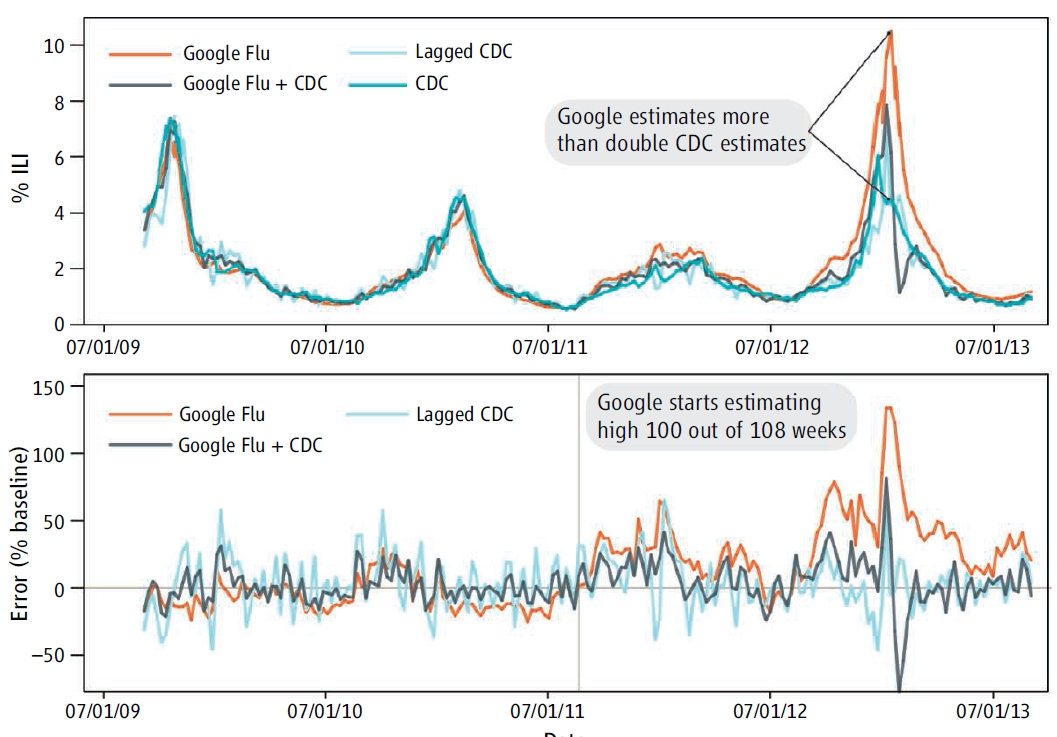
\includegraphics[width=8cm]{c:/Users/joon/Sync/Org-Coursepack/Assets/Images/Big_Data/Google_Flu_Trends.jpg}
\end{center}

(source: \href{http://www.uvm.edu/\~cdanfort/csc-reading-group/lazer-flu-science-2014.pdf}{The Parable of Google Flu: Traps in Big Data Analysis})

\subsubsection{What Went Wrong?}
\label{sec:org5a33904}

\begin{itemize}
\item Quality of search terms

\begin{itemize}
\item \textbf{influenza-like illness}
\end{itemize}

\item Prediction without theory

\(\Rightarrow\) overfitting problem
\end{itemize}
\subsection{Overfitting}
\label{sec:orgabcf212}
\subsubsection{Error Term in Regression}
\label{sec:orge23c055}
\begin{itemize}
\item When we think about typical regression model:

\[ y_{i} = \beta_{0} + \beta_{1}x_{i1} + \cdots + \beta_{K}x_{iK} + \varepsilon_{i} \]

\item The error term (\(\varepsilon_{i}\)) is supposed to have mean zero
\item Not \emph{predictable}
\item However, once they are realized, one can often find some pattern in them,
which will disappear as more data accumulate
\begin{itemize}
\item e.g., stock prices are supposed to be random-walk; however, from historical data, 
patterns will pop up
\end{itemize}
\end{itemize}
\subsubsection{Google Flu and Overfitting}
\label{sec:org9b99f1f}
Find the best matches among 50 million search terms to fit 1152 data points

"They \ldots{} overfit the data. They had fifty million search terms, and they
found some that happened to fit the frequency of the 'flu' over the
preceding decade or so, but really they were getting idiosyncratic terms
that were peaking in the winter at the time the 'flu' peaks \ldots{} but wasn't
driven by the fact that people were actually sick with the 'flu',"

(David Lazer, an interview with \href{http://www.sciencemag.org/content/343/6176/1270.2.full}{Science})
\subsection{Takeaways}
\label{sec:org6707529}
\begin{itemize}
\item Be careful of "overfitting", especially when you have a lot of variables
\item Conduct out-of-sample validation
\end{itemize}
\subsection{Out-of-Sample Validation}
\label{sec:org7db504c}
\begin{itemize}
\item Use only a subset of data (e.g., 80\% of the sample; train dataset) to estimate coefficients
\item Then predict \(\hat{y}_i\) values for the rest of the sample (validation
dataset) using the estimated coefficients and actual data for \(x_{k}\)'s
as if we do not know actual \(y_{i}\):

\[ \hat{y}_{i}= \hat{\beta}_{0} + \hat{\beta}_{1} x_{1i} +
      \hat{\beta}_{2} x_{2i} + \cdots + \hat{\beta}_{K} x_{Ki} \]

\item Compare \(\hat{y}_{i}\) and the actual \(y_{i}\)
\end{itemize}
\end{document}